% !TEX program = xelatex
% ============================================================
% 《电磁场与电磁波》课程论文 —— 课题一：圆形线圈
% 编译：xelatex -> bibtex -> xelatex -> xelatex
% 数据来源：matlab/paper_circular_coil/ 下脚本的实际运行结果
% ============================================================
\documentclass[zihao=-4,a4paper]{ctexart}

\usepackage[margin=2.5cm]{geometry}
\usepackage{amsmath,amssymb}
\usepackage{graphicx}
\usepackage{booktabs}
\usepackage{array}
\usepackage{caption}
\usepackage{subcaption}
\usepackage{siunitx}
\usepackage{xcolor}
\usepackage{listings}
\usepackage[colorlinks,linkcolor=black,citecolor=black,urlcolor=blue]{hyperref}

\graphicspath{{figures/}}

\lstdefinestyle{mat}{
  language=Matlab, basicstyle=\ttfamily\footnotesize, keywordstyle=\bfseries,
  commentstyle=\itshape\color{black!60}, stringstyle=\color{black!60},
  numbers=left, numberstyle=\tiny\color{black!50}, xleftmargin=2.2em,
  breaklines=true, frame=single, framerule=0.3pt, rulecolor=\color{black!40},
  showstringspaces=false, tabsize=2, columns=flexible, keepspaces=true
}

% ---------- 论文信息 ----------
\newcommand{\papertitle}{圆形经颅磁刺激线圈的磁场计算与有限元仿真对比分析}
\newcommand{\paperauthor}{（姓名、学号待填）}
\newcommand{\paperdate}{2026 年 9 月}

\title{\heiti \papertitle}
\author{\paperauthor \\ \small 《电磁场与电磁波》课程论文（课题一：圆形线圈）}
\date{\paperdate}

\begin{document}

\maketitle

% ============================================================
\begin{abstract}
经颅磁刺激（TMS）是一种无创刺激神经组织的电磁技术，刺激线圈的空间磁场
分布直接决定刺激的位置与聚焦性。本文针对课题一给出的圆形线圈（平面螺旋、
双层各 9 匝、外径 \SI{115}{mm}、内径 \SI{30}{mm}、总厚度小于 \SI{10}{mm}），
建立了基于毕奥--萨伐尔定律的磁场计算模型：将绕组离散为 4320 个直线电流
单元，采用直线段磁场闭式表达式逐段叠加求解空间磁场；推导了单匝圆环离轴
磁场的完整椭圆积分表达式作为验证基准。MATLAB 数值计算结果表明：归一化
电流 \SI{1}{A} 时线圈中心处磁感应强度为 \SI{351.29}{\micro T}，其轴向分
布与多匝圆环解析解的最大相对偏差为 0.27\%，离轴场与椭圆积分精确解的峰值
归一偏差为 $2.3\times10^{-4}$；线圈下方 \SI{10}{mm} 处磁感应强度峰值衰减
为中心值的 77.7\%，径向半高全宽由绕组内的 \SI{30}{mm} 增大至深处的约
\SI{70}{mm}，表明圆形线圈聚焦性随深度增加而变差；引线对磁场的贡献在轴线
上不超过 0.42\%。采用有限元软件 FEMM 建立轴对称静磁场模型（91\,651 个一
阶三角形单元，圆弧外边界施加渐近混合边界条件）进行对比，两者轴线磁场的
均方根相对偏差为 0.44\%、最大偏差 1.02\%，径向分布峰值偏差 0.29\%，相互
验证了计算模型的正确性。

\vspace{1em}
\noindent\textbf{关键词：} 经颅磁刺激；圆形线圈；毕奥--萨伐尔定律；椭圆
积分；磁场分布；有限元法；FEMM
\end{abstract}

\tableofcontents
\bigskip

% ============================================================
\section{简介}\label{sec:intro}

经颅磁刺激（Transcranial Magnetic Stimulation, TMS）利用时变磁场穿透颅骨
在大脑皮层感应出涡流，从而无创地兴奋或抑制神经组织，自 1985 年 Barker 等
首次实现人体运动皮层磁刺激以来\cite{barker1985}，已成为抑郁症等疾病的
临床治疗手段和脑功能研究的重要工具\cite{rossini2015}。刺激线圈是 TMS
装置的核心部件，其结构决定了空间磁场的分布，进而决定刺激位置、深度与聚
焦性：最早的圆形线圈结构简单、刺激面积大但聚焦性差，而后续出现的 8 字
线圈正是通过两个反接圆形线圈的组合来提高聚焦性\cite{ueno1988}。

本文以课题一的圆形线圈为对象，完成以下工作：
（1）基于毕奥--萨伐尔定律建立圆形线圈的磁场计算模型，推导直线电流单元
的闭式磁场表达式与单匝圆环离轴磁场的椭圆积分精确解；
（2）编写 MATLAB 程序，计算线圈的轴线磁场、径向分布、截面云图与磁力线，
量化其聚焦性随深度的变化，并对引线的影响进行对比分析；
（3）采用有限元软件 FEMM 建立轴对称静磁场模型，将有限元解与数值解进行
对比，分析偏差来源，验证计算模型的正确性。

本文结构安排如下：第 \ref{sec:model} 节给出理论分析与计算模型；
第 \ref{sec:matlab} 节介绍 MATLAB 计算方法与代码实现；
第 \ref{sec:results} 节给出计算结果与分析；
第 \ref{sec:fem} 节介绍有限元仿真及其与数值结果的对比；
第 \ref{sec:conclusion} 节给出结论。

% ============================================================
\section{理论分析与计算模型}\label{sec:model}

\subsection{毕奥--萨伐尔定律与直线电流单元的闭式解}

载流导线元 $\mathrm{d}\boldsymbol{l}$ 在空间场点 $\boldsymbol{r}$ 处产生
的磁感应强度服从毕奥--萨伐尔定律：
\begin{equation}
  \mathrm{d}\boldsymbol{B}
  = \frac{\mu_0}{4\pi}\,\frac{I\,\mathrm{d}\boldsymbol{l}\times\hat{\boldsymbol{R}}}{R^2},
  \qquad
  \boldsymbol{B}(\boldsymbol{r}) = \frac{\mu_0 I}{4\pi}
  \oint_l \frac{\mathrm{d}\boldsymbol{l}\times\boldsymbol{R}}{R^3},
  \label{eq:bs}
\end{equation}
其中 $\mu_0 = 4\pi\times10^{-7}\,\mathrm{H/m}$ 为真空磁导率，
$\boldsymbol{R} = \boldsymbol{r}-\boldsymbol{r}'$ 为源点指向场点的矢量。
多匝线圈的总场为各匝贡献的矢量和。

数值计算中，将任意折线状载流导线剖分为有限长的直线单元。对两端点为
$A$、$B$ 的直线单元（单元矢量 $\boldsymbol{d}=\boldsymbol{B}-\boldsymbol{A}$，
场点相对两端点的矢量为 $\boldsymbol{R}_1$、$\boldsymbol{R}_2$），式
\eqref{eq:bs} 的积分存在闭式解：
\begin{equation}
  \boldsymbol{B} = \frac{\mu_0 I}{4\pi}\,
  \frac{\boldsymbol{R}_1\times\boldsymbol{R}_2}
       {\left|\boldsymbol{R}_1\times\boldsymbol{R}_2\right|^2}\,
  \boldsymbol{d}\cdot
  \left(\frac{\boldsymbol{R}_1}{R_1} - \frac{\boldsymbol{R}_2}{R_2}\right).
  \label{eq:seg}
\end{equation}
相比对单元做中点近似，式~\eqref{eq:seg} 对每一单元精确积分，剖分误差仅
来自以弦代弧的几何离散，因而收敛极快（见第 \ref{sec:results} 节）。

\subsection{单匝圆环磁场的解析解}

半径为 $a$ 的单匝圆环载流 $I$，取圆环轴线为 $z$ 轴，轴线上距环心 $z$ 处
的磁场有熟知的解析解：
\begin{equation}
  B_z(z) = \frac{\mu_0 I a^2}{2\,(a^2+z^2)^{3/2}},
  \qquad
  B_z(0) = \frac{\mu_0 I}{2a}.
  \label{eq:loop-axis}
\end{equation}
离轴场可用第一、二类完全椭圆积分表示\cite{smythe1989,jackson1999}。记
$s=\sqrt{(a+\rho)^2+z^2}$，$Q=(a-\rho)^2+z^2$，$k^2 = 4a\rho/s^2$，则
圆柱坐标下场点 $(\rho,z)$ 处的两个分量为
\begin{align}
  B_\rho &= \frac{\mu_0 I z}{2\pi \rho\, s}
            \left[ -K(k) + \frac{a^2+\rho^2+z^2}{Q}\,E(k) \right],
  \label{eq:brho}\\
  B_z    &= \frac{\mu_0 I}{2\pi s}
            \left[ K(k) + \frac{a^2-\rho^2-z^2}{Q}\,E(k) \right],
  \label{eq:bz}
\end{align}
其中 $K(k)=\int_0^{\pi/2}(1-k^2\sin^2\theta)^{-1/2}\mathrm{d}\theta$，
$E(k)=\int_0^{\pi/2}(1-k^2\sin^2\theta)^{1/2}\mathrm{d}\theta$。本文按
算术--几何平均（AGM）迭代自实现 $K$、$E$ 的双精度计算，不依赖商业工具
箱；$\rho\to 0$ 时式~\eqref{eq:brho}、\eqref{eq:bz} 退化为轴线解
式~\eqref{eq:loop-axis}。该精确解用于验证数值计算内核（第
\ref{sec:matlab} 节）。

\subsection{线圈几何模型与参数}

课题一线圈为平面螺旋结构：绕组沿阿基米德螺旋线从内径绕到外径，双层同向
串联。以线圈中平面为 $xy$ 平面、轴线为 $z$ 轴建立圆柱坐标系
$(\rho,\varphi,z)$，第 $k$ 层螺旋线为
\begin{equation}
  \rho(\theta) = r_\mathrm{in} + (r_\mathrm{out}-r_\mathrm{in})\,\frac{\theta}{2\pi N},
  \quad \theta\in[0,\,2\pi N],\quad z = z_k,
  \label{eq:spiral}
\end{equation}
其中 $N=9$ 为每层匝数，$z_k$ 为第 $k$ 层所在高度。由图纸参数与 $\Phi 4$
紫铜管绕组的几何关系确定的模型参数见表~\ref{tab:param}。

\begin{table}[htbp]
  \centering
  \caption{圆形线圈图纸参数与计算模型参数}
  \label{tab:param}
  \begin{tabular}{llll}
    \toprule
    参数 & 符号 & 数值 & 说明 \\
    \midrule
    线圈外径 & $D_\mathrm{out}$ & \SI{115}{mm} & 图纸标称值（注明略小，不影响计算） \\
    线圈内径 & $D_\mathrm{in}$  & \SI{30}{mm}  & 图纸（$\pm 1$） \\
    层数 $\times$ 每层匝数 & --- & $2\times 9$ & 图纸 \\
    总匝数 & $N_\mathrm{t}$ & 18 & 图纸 \\
    径向绕距 & $\Delta a$ & \SI{4.72}{mm} & $(r_\mathrm{out}-r_\mathrm{in})/N = 42.5/9$ \\
    层间距离 & $h$ & \SI{4}{mm} & 取 $\Phi 4$ 紫铜管外径 \\
    线圈总厚度 & --- & $\approx\SI{8}{mm}(<\SI{10}{mm})$ & 与图纸侧视图一致 \\
    激励电流 & $I$ & \SI{1}{A} & 归一化，结果随 $I$ 线性缩放 \\
    \bottomrule
  \end{tabular}
\end{table}

计算采用如下简化假设：
（1）\textbf{准静态近似}：TMS 激励电流的变化时间为百微秒量级，对应电磁
波长远大于线圈尺寸，可按恒定电流磁场处理；
（2）\textbf{灯丝（线电流）近似}：将每匝电流集中到管的中心线上，绕组截
面分布的影响将在第 \ref{sec:fem} 节通过有限元模型定量评估；
（3）\textbf{不计铁磁材料与涡流}：线圈周围为空气，无磁路；
（4）\textbf{引线单独建模}：主模型只含螺旋绕组；引线对（两条平行反流直
导线，间距 \SI{18}{mm}、长 \SI{100}{mm}，$\mathrm{R}20$ 弯头未计入）作为
独立工况对比计算，见第 \ref{sec:results} 节。

由此，总磁场为双层螺旋各匝贡献之和：
\begin{equation}
  \boldsymbol{B}(\rho,z) = \sum_{k=1}^{2}\sum_{j=1}^{9} \boldsymbol{B}_{k,j}(\rho,z).
  \label{eq:superpose}
\end{equation}

% ============================================================
\section{运用 MATLAB 进行计算及代码}\label{sec:matlab}

\subsection{程序结构}

计算程序由通用磁场计算库与论文驱动脚本两部分组成，全部代码随论文提交，
文件清单见表~\ref{tab:code}。运行环境为 MATLAB R2026a，无附加工具箱依赖
（椭圆积分按 AGM 算法自实现）。

\begin{table}[htbp]
  \centering
  \caption{MATLAB 程序文件清单}
  \label{tab:code}
  \begin{tabular}{ll}
    \toprule
    文件 & 功能 \\
    \midrule
    \texttt{common/spiral\_pts.m}          & 阿基米德平面螺旋线离散 \\
    \texttt{common/multilayer\_spiral.m}   & 多层螺旋绕组生成（含层间串联方向处理） \\
    \texttt{common/bs\_field.m}            & 直线单元闭式毕奥--萨伐尔磁场核（式~\eqref{eq:seg}） \\
    \texttt{common/field\_on\_axis.m}      & 轴线磁场采样 \\
    \texttt{common/field\_on\_plane.m}     & 平面磁场采样 \\
    \texttt{common/coil\_L\_R.m}           & 电感（Neumann 积分）与直流电阻估算 \\
    \texttt{paper\_circular\_coil/elliptic\_ke.m}       & AGM 完全椭圆积分 $K$、$E$ \\
    \texttt{paper\_circular\_coil/loop\_field\_elliptic.m} & 单匝圆环离轴场精确解（式~\eqref{eq:brho}\eqref{eq:bz}） \\
    \texttt{paper\_circular\_coil/main\_paper\_figures.m}  & 主脚本：全部图件、指标与数据导出 \\
    \texttt{paper\_circular\_coil/run\_femm\_axis.m}       & FEMM 轴对称模型自动建模与求解 \\
    \texttt{paper\_circular\_coil/compare\_femm.m}         & 有限元解与数值解对比 \\
    \bottomrule
  \end{tabular}
\end{table}

\subsection{离散化与计算流程}

每匝螺旋按 \texttt{nPer} $=240$ 个圆周角等分点离散为折线（双层共
$2\times9\times240 = 4320$ 个直线单元），磁场核按式~\eqref{eq:seg} 逐单
元精确叠加。计算流程为：由表~\ref{tab:param} 生成绕组几何 $\rightarrow$
按式~\eqref{eq:seg} 叠加求指定场点的 $\boldsymbol{B}
\rightarrow$ 与解析解校验 $\rightarrow$ 输出轴线/径向/平面/截面分布及聚
焦性指标。磁场核的核心实现如下（完整代码见提交件）：

\begin{lstlisting}[style=mat, caption={磁场核 \texttt{bs\_field.m} 核心语句（式~\eqref{eq:seg}）}]
R1 = P - A3;                 % p x S x 3, field point to segment start
R2 = P - B3;                 % p x S x 3, field point to segment end
C  = cross(R1,R2,3);         % R1 x R2
c2 = sum(C.^2,3);            % |R1 x R2|^2
u1 = R1./r1;  u2 = R2./r2;
fv = sum(d3.*(u1-u2),3);     % d . (R1/|R1| - R2/|R2|)
Bv = squeeze(sum(C.*(fv./c2).*I3, 2));   % sum over segments
B(ii,:) = (mu0/(4*pi))*Bv;
\end{lstlisting}

\subsection{验证策略与收敛性}

数值结果通过两条独立途径验证：
（1）\textbf{轴线磁场}与每匝取平均半径的\textbf{多匝圆环解析解}
（对每匝按式~\eqref{eq:loop-axis} 叠加）对比；
（2）\textbf{单匝圆环离轴场}与椭圆积分精确解
（式~\eqref{eq:brho}\eqref{eq:bz}）对比。

离散收敛性见表~\ref{tab:conv}：随每匝离散段数 $\mathtt{nPer}$ 增大，轴
线磁场与解析解的偏差由 $3.5\times10^{-3}$（60 段）降至 $2.6\times10^{-3}$
（960 段）并趋于饱和，该饱和值是螺旋绕组与「平均半径圆环」两种模型本身
的几何差别（半绕距内半径线性增长所致），而非离散误差；离散误差本身由单
匝圆环测试分离——240 段离散下，数值核与椭圆积分精确解的峰值归一偏差仅
$2.3\times10^{-4}$（$B_z$）与 $1.6\times10^{-4}$（$B_\rho$），已充分收敛，
故后续计算取 $\mathtt{nPer}=240$。

\begin{table}[htbp]
  \centering
  \caption{离散收敛性：轴线磁场与多匝圆环解析解的最大相对偏差}
  \label{tab:conv}
  \begin{tabular}{cccccc}
    \toprule
    $\mathtt{nPer}$（段/匝） & 60 & 120 & 240 & 480 & 960 \\
    \midrule
    最大相对偏差 & $3.52\times10^{-3}$ & $2.85\times10^{-3}$ &
    $2.68\times10^{-3}$ & $2.63\times10^{-3}$ & $2.62\times10^{-3}$ \\
    \bottomrule
  \end{tabular}
\end{table}

% ============================================================
\section{结果分析}\label{sec:results}

\subsection{线圈模型与轴线磁场}

图~\ref{fig:model} 给出按式~\eqref{eq:spiral} 生成的线圈模型。图
\ref{fig:axis}（a）为归一化电流 \SI{1}{A} 下的轴线磁场分布：线圈中心处
$B_z(0,0) = \SI{351.29}{\micro T}$；由于双层绕组分别位于 $z=0$ 与
$z=\SI{4}{mm}$，轴线峰值 $B_z = \SI{354.34}{\micro T}$ 出现在两层之间
（$z=\SI{+2}{mm}$）处。数值解与多匝圆环解析解在整个采样区间内的曲线完全
重合，相对偏差最大 0.27\%（图~\ref{fig:axis}(b)），与表~\ref{tab:conv}
一致。

\begin{figure}[htbp]
  \centering
  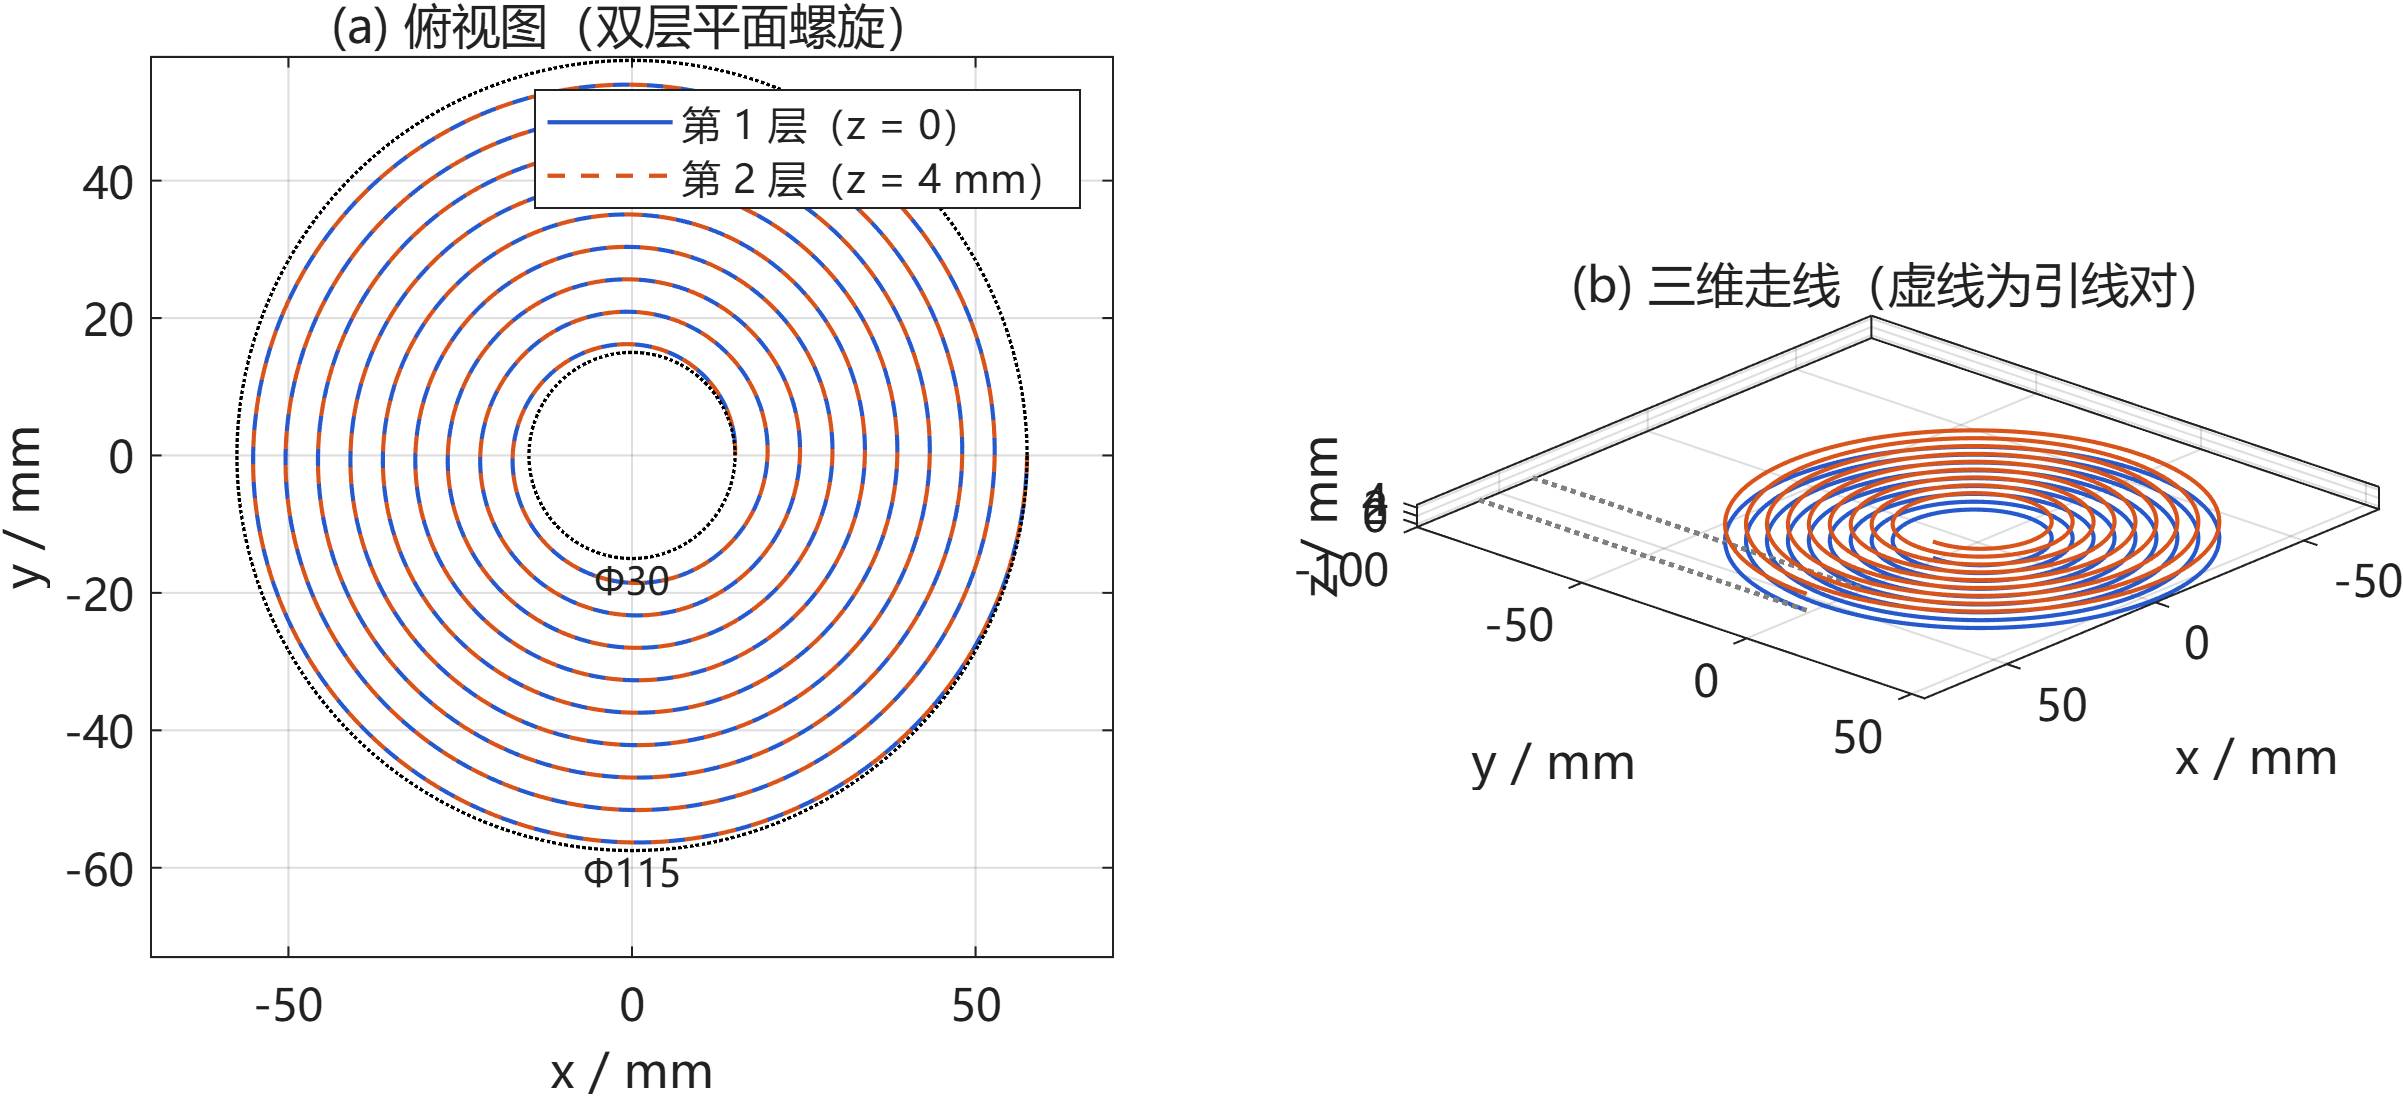
\includegraphics[width=0.98\textwidth]{fig01_model.png}
  \caption{圆形线圈计算模型：(a) 俯视图（双层平面螺旋，虚线圆为内外径）；
    (b) 三维走线（灰色虚线为引线对模型）}
  \label{fig:model}
\end{figure}

\begin{figure}[htbp]
  \centering
  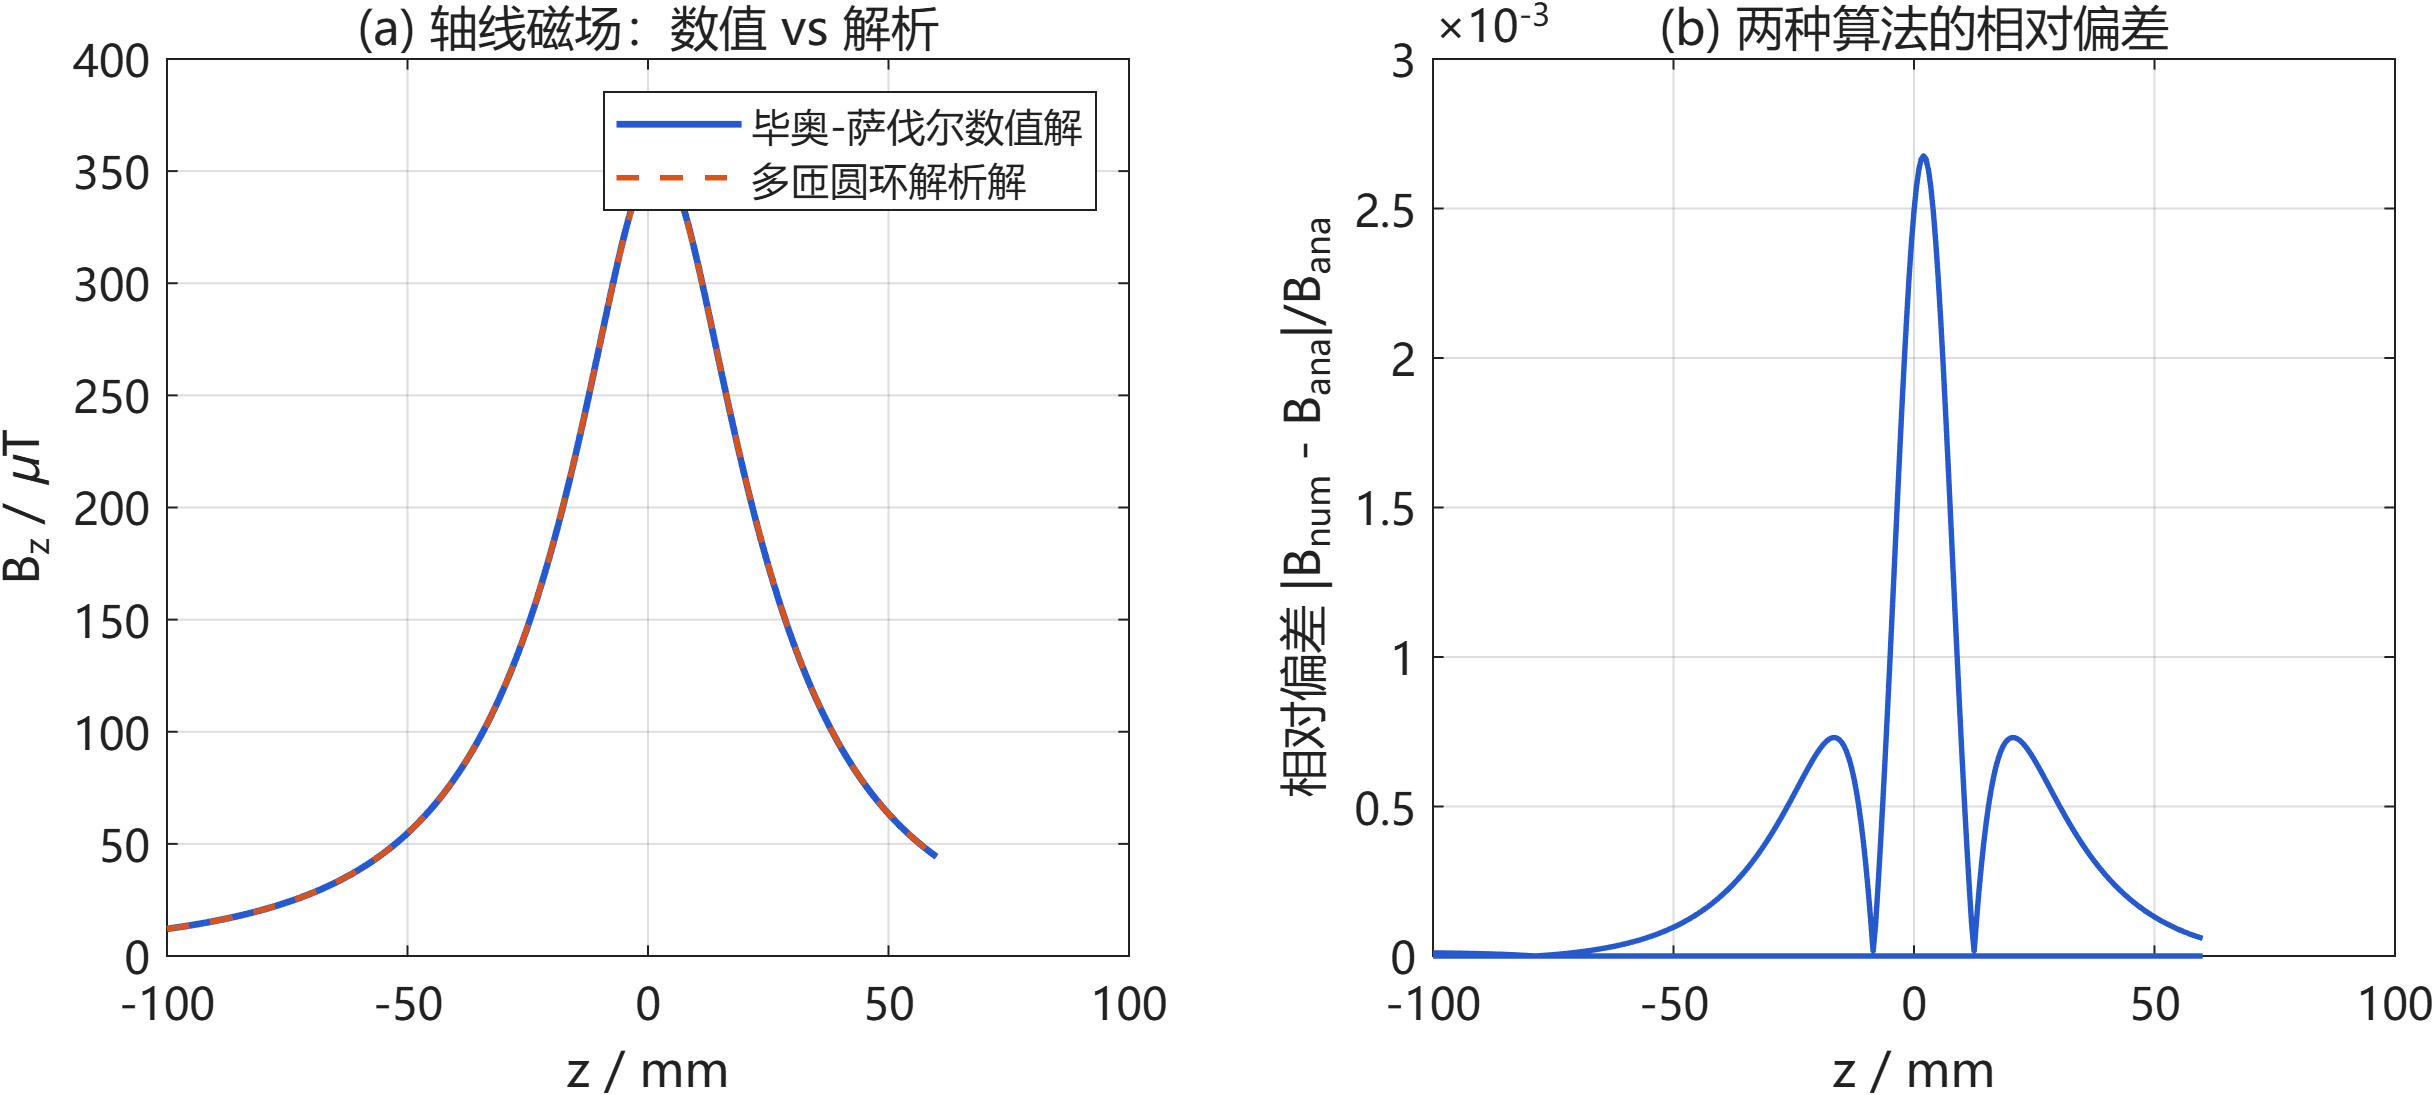
\includegraphics[width=0.98\textwidth]{fig02_axis_validation.png}
  \caption{轴线磁场：数值解与多匝圆环解析解的对比（a）及相对偏差（b）}
  \label{fig:axis}
\end{figure}

\subsection{离轴磁场的椭圆积分验证}

图~\ref{fig:elliptic} 给出单匝圆环（$a=\SI{36.25}{mm}$）在 $z=\SI{-10}{mm}$
平面上的离轴磁场：数值解与椭圆积分精确解的曲线在整个 $\rho$ 范围内重合，
$B_z$、$B_\rho$ 的峰值归一最大偏差分别为 $2.3\times10^{-4}$ 与
$1.6\times10^{-4}$，验证了磁场核在离轴区域的正确性。

\begin{figure}[htbp]
  \centering
  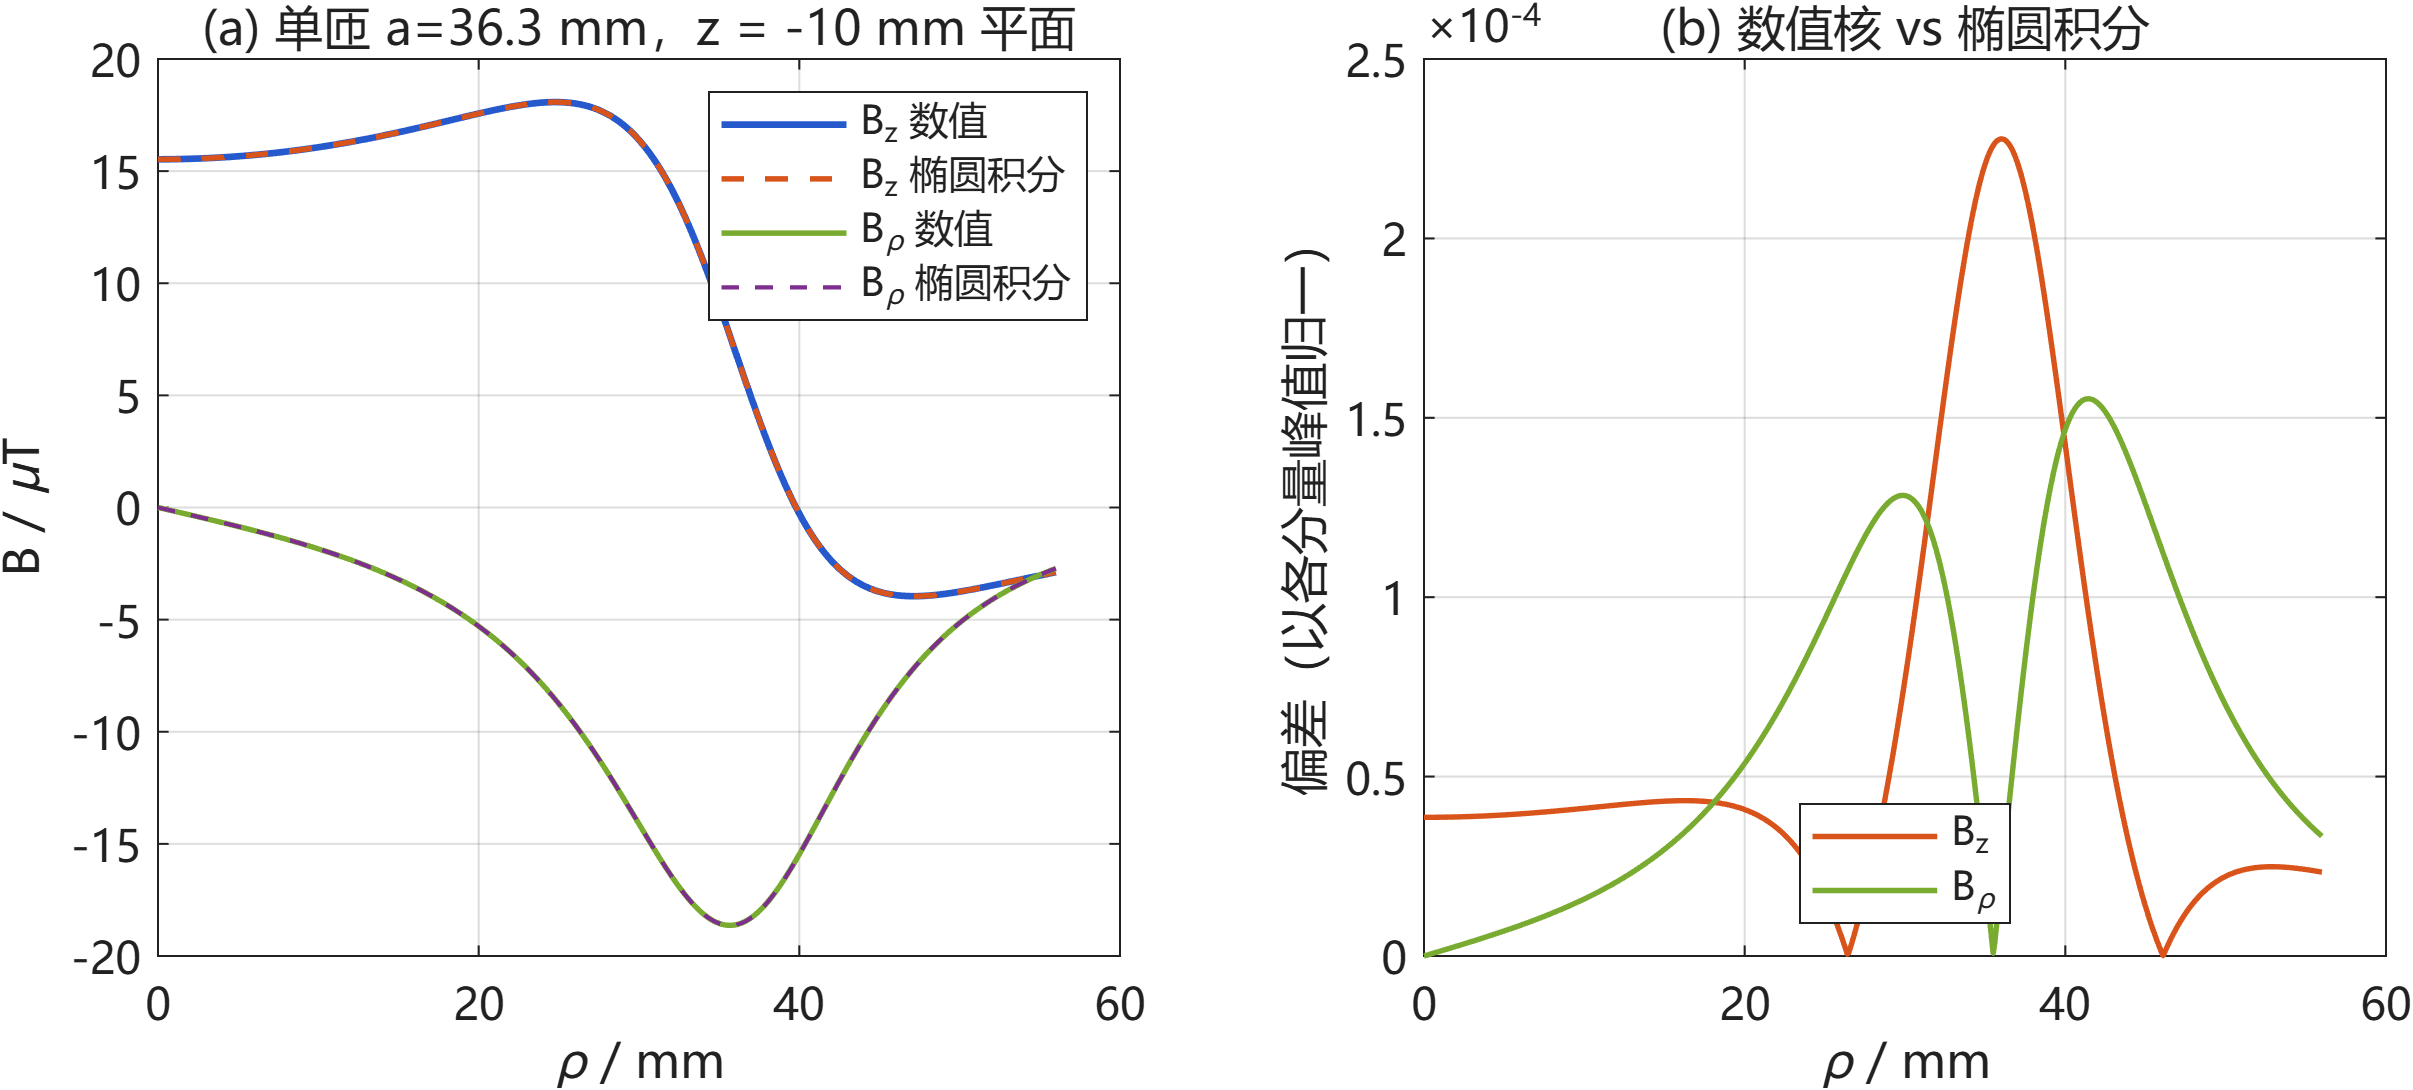
\includegraphics[width=0.98\textwidth]{fig03_elliptic_validation.png}
  \caption{单匝圆环离轴磁场：直线单元数值解与椭圆积分精确解的对比（a）
    及峰值归一偏差（b）}
  \label{fig:elliptic}
\end{figure}

\subsection{空间磁场分布}

图~\ref{fig:plane} 为线圈下方 $z=\SI{-10}{mm}$ 处（模拟线圈表面与头皮间
距）的 $B_z$ 分布：磁感应强度在线圈投影区内近似平台状分布，峰值
\SI{273.85}{\micro T} 位于线圈中心，为线圈中心值的 77.7\%；绕组正下方
梯度最大。图~\ref{fig:rz} 的 $r$--$z$ 半平面截面给出磁感应强度模值的空
间衰减与磁力线闭合回路：磁通全部穿过线圈孔洞后绕过绕组外侧返回，轴向衰
减显著快于径向扩散。

\begin{figure}[htbp]
  \centering
  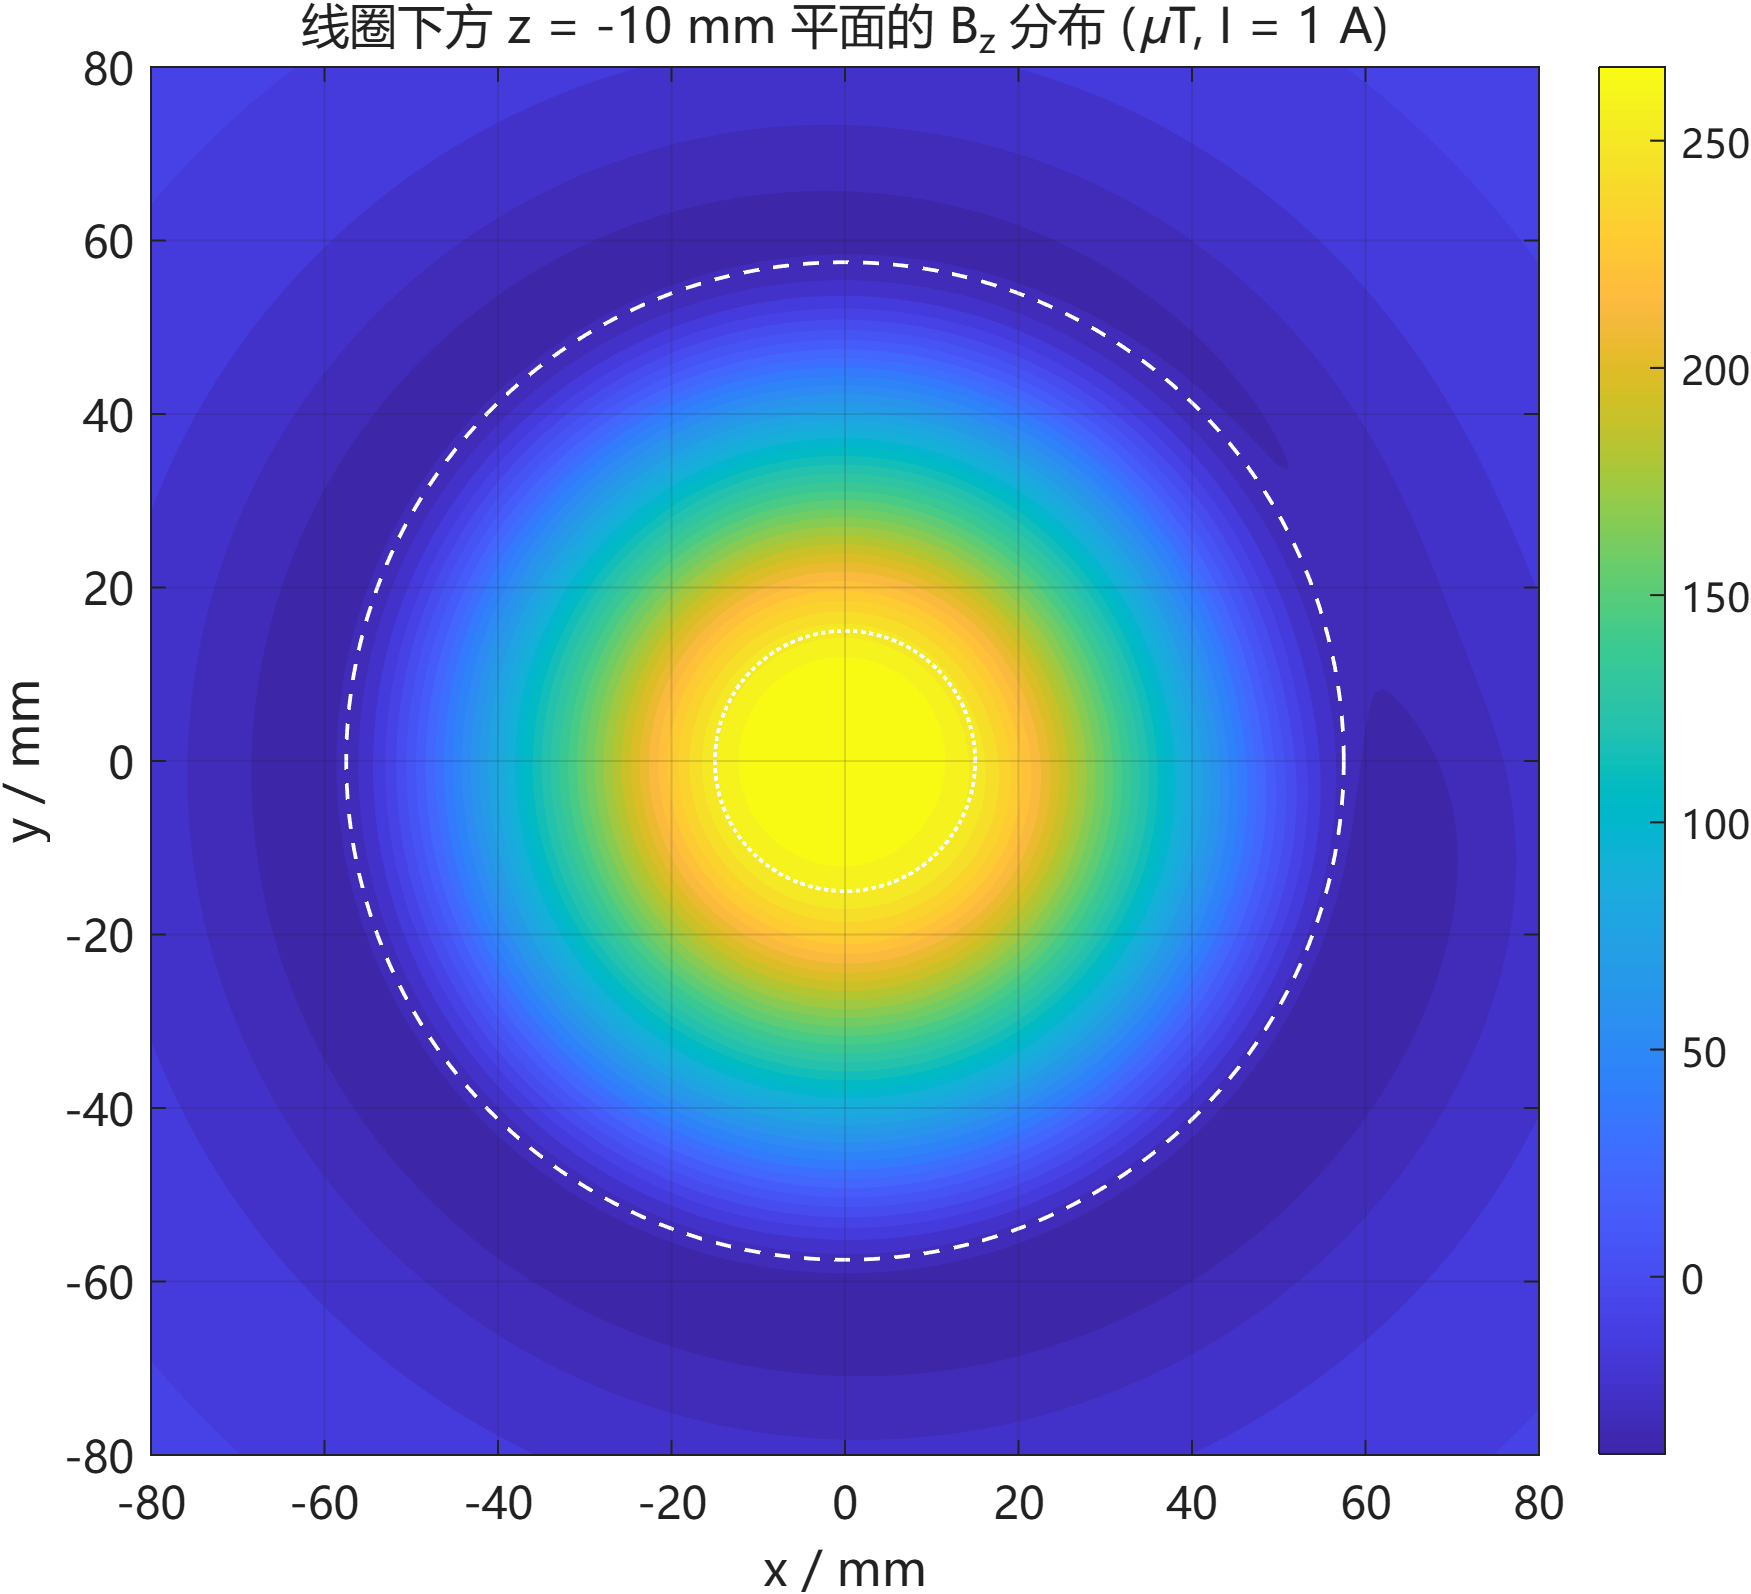
\includegraphics[width=0.72\textwidth]{fig04_plane_Bz.png}
  \caption{线圈下方 $z=\SI{-10}{mm}$ 平面的 $B_z$ 分布（\SI{1}{A}）}
  \label{fig:plane}
\end{figure}

\begin{figure}[htbp]
  \centering
  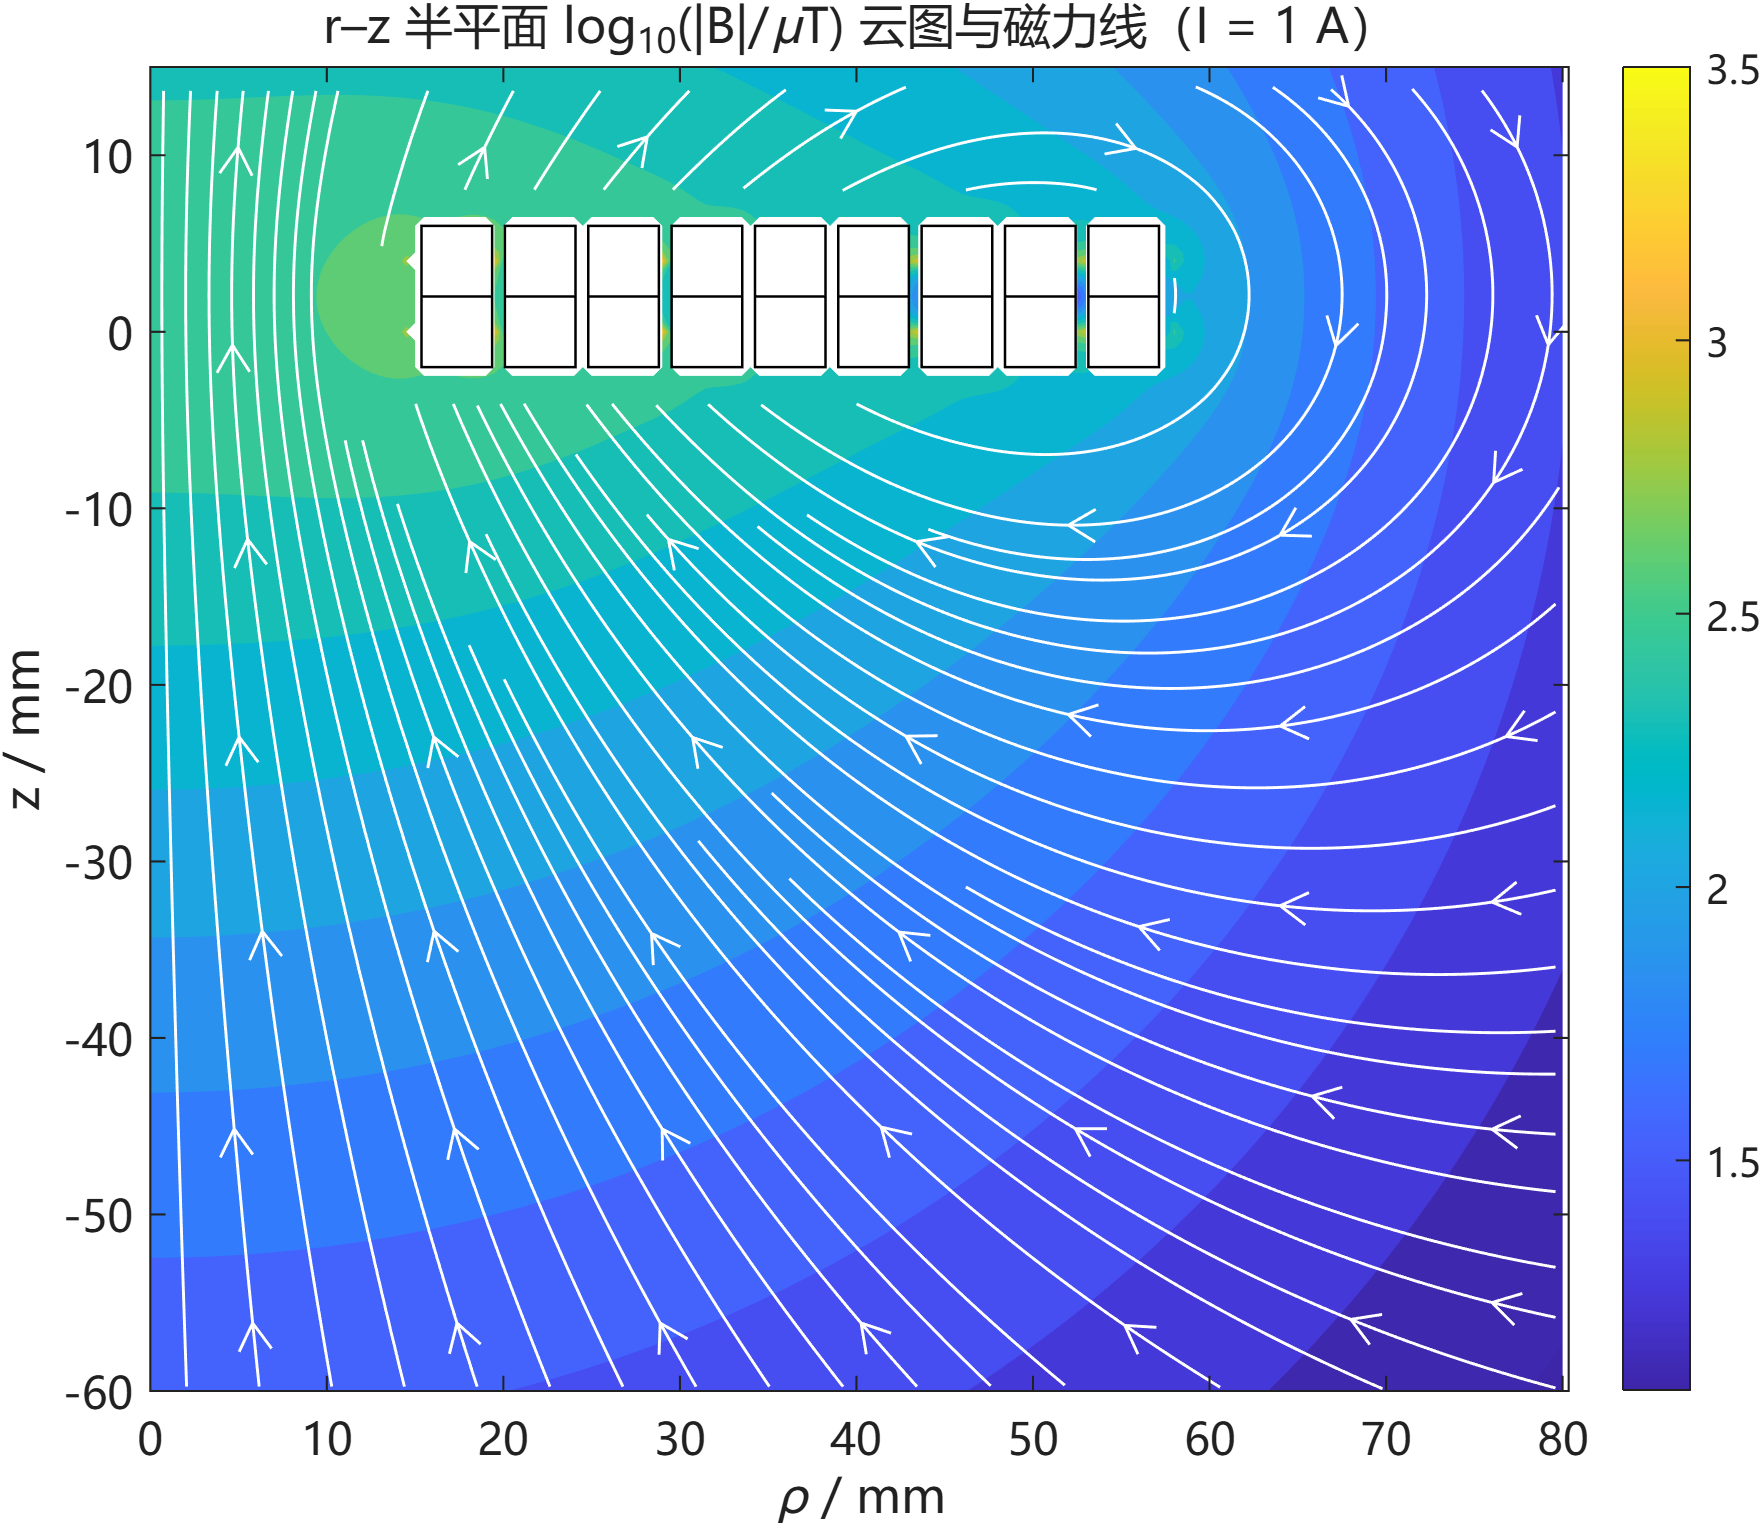
\includegraphics[width=0.82\textwidth]{fig05_rz_section.png}
  \caption{$r$--$z$ 半平面 $\log_{10}(|B|/\si{\micro T})$ 云图与磁力线
    （白色矩形为绕组截面，\SI{1}{A}）}
  \label{fig:rz}
\end{figure}

\subsection{聚焦性随深度的变化}

以轴线峰值衰减一半定义的径向半高全宽（FWHM）随深度的变化见
图~\ref{fig:focality} 与表~\ref{tab:fwhm}：线圈平面内 $B_z$ 的半高宽仅
\SI{30}{mm}（受绕组内径限制）；离开线圈后迅速展宽至 \SI{65}--\SI{70}{mm}
并随深度缓慢增大。轴向衰减方面，$z=\SI{-25}{mm}$ 处轴线峰值降为中心值的
41.8\%，半衰深度约 \SI{27}{mm}。可见圆形线圈的磁场随深度增加快速衰减且
半高宽不断增大——刺激深度与聚焦性不可兼得，这正是后续 8 字形等多 focusing
线圈构型改进的出发点。

\begin{table}[htbp]
  \centering
  \caption{不同深度的轴线峰值与径向半高全宽（\SI{1}{A}）}
  \label{tab:fwhm}
  \begin{tabular}{cccccccc}
    \toprule
    深度 $z$ / mm & 0 & $-5$ & $-10$ & $-15$ & $-20$ & $-25$ & $-30$ \\
    \midrule
    轴线峰值 / \si{\micro T} & 351.29 & 320.80 & 272.87 & 224.07 & 181.67 & 146.99 & 119.26 \\
    相对线圈中心 & 100\% & 91.3\% & 77.7\% & 63.8\% & 51.7\% & 41.8\% & 33.9\% \\
    径向 FWHM / mm & 30.0 & 67.1 & 65.9 & 66.0 & 67.0 & 68.4 & 70.4 \\
    \bottomrule
  \end{tabular}
\end{table}

\begin{figure}[htbp]
  \centering
  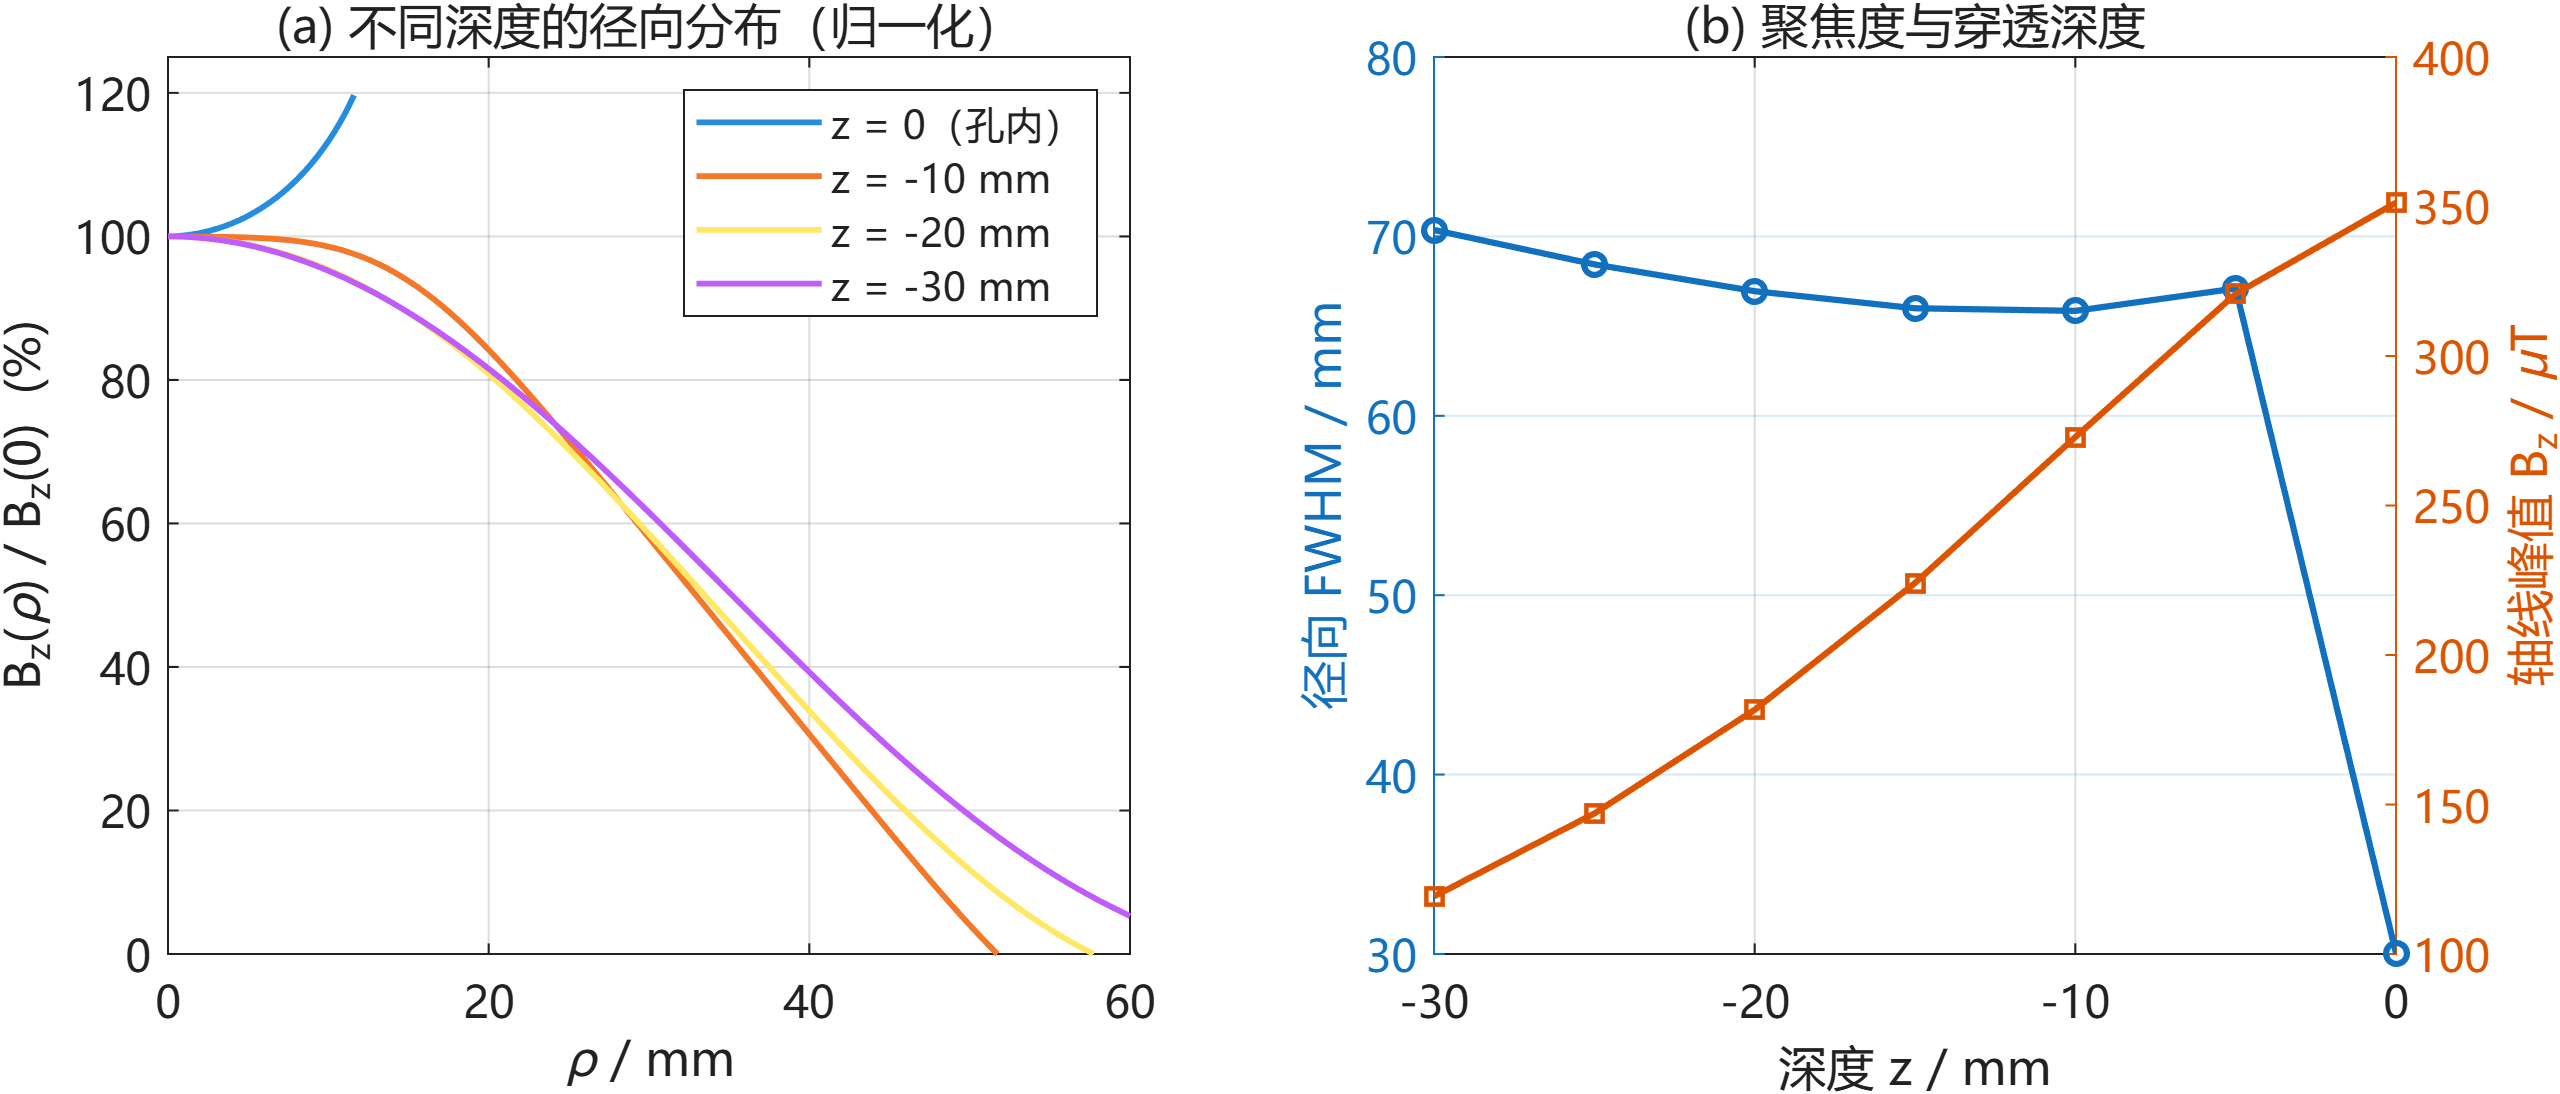
\includegraphics[width=0.98\textwidth]{fig07_focality.png}
  \caption{聚焦性分析：(a) 不同深度的径向分布（归一化）；(b) 径向 FWHM
    与轴线峰值随深度的变化}
  \label{fig:focality}
\end{figure}

\subsection{引线的影响}

图纸中绕组经 $\mathrm{R}20$ 弯颈部向下引出两根引线至手柄。将引线建模为
两条平行反流直导线（间距 \SI{18}{mm}、长 \SI{100}{mm}），与不含引线的模
型对比（图~\ref{fig:leads}）：轴线上磁感应强度的最大绝对变化仅
\SI{846.95}{nT}，约为该处磁场的 0.42\%；$z=\SI{-10}{mm}$ 平面磁感应强度
峰值的相对变化为 0.19\%（\SI{277.59}{\micro T} $\rightarrow$
\SI{278.13}{\micro T}）。这是由于两根引线电流等大反向、相距较近，其磁场
在远大于线间距处大部分自相抵消。因此后续磁场分析与有限元建模均忽略引线，
其影响量级（$<0.5\%$）远小于工程关注精度。

\begin{figure}[htbp]
  \centering
  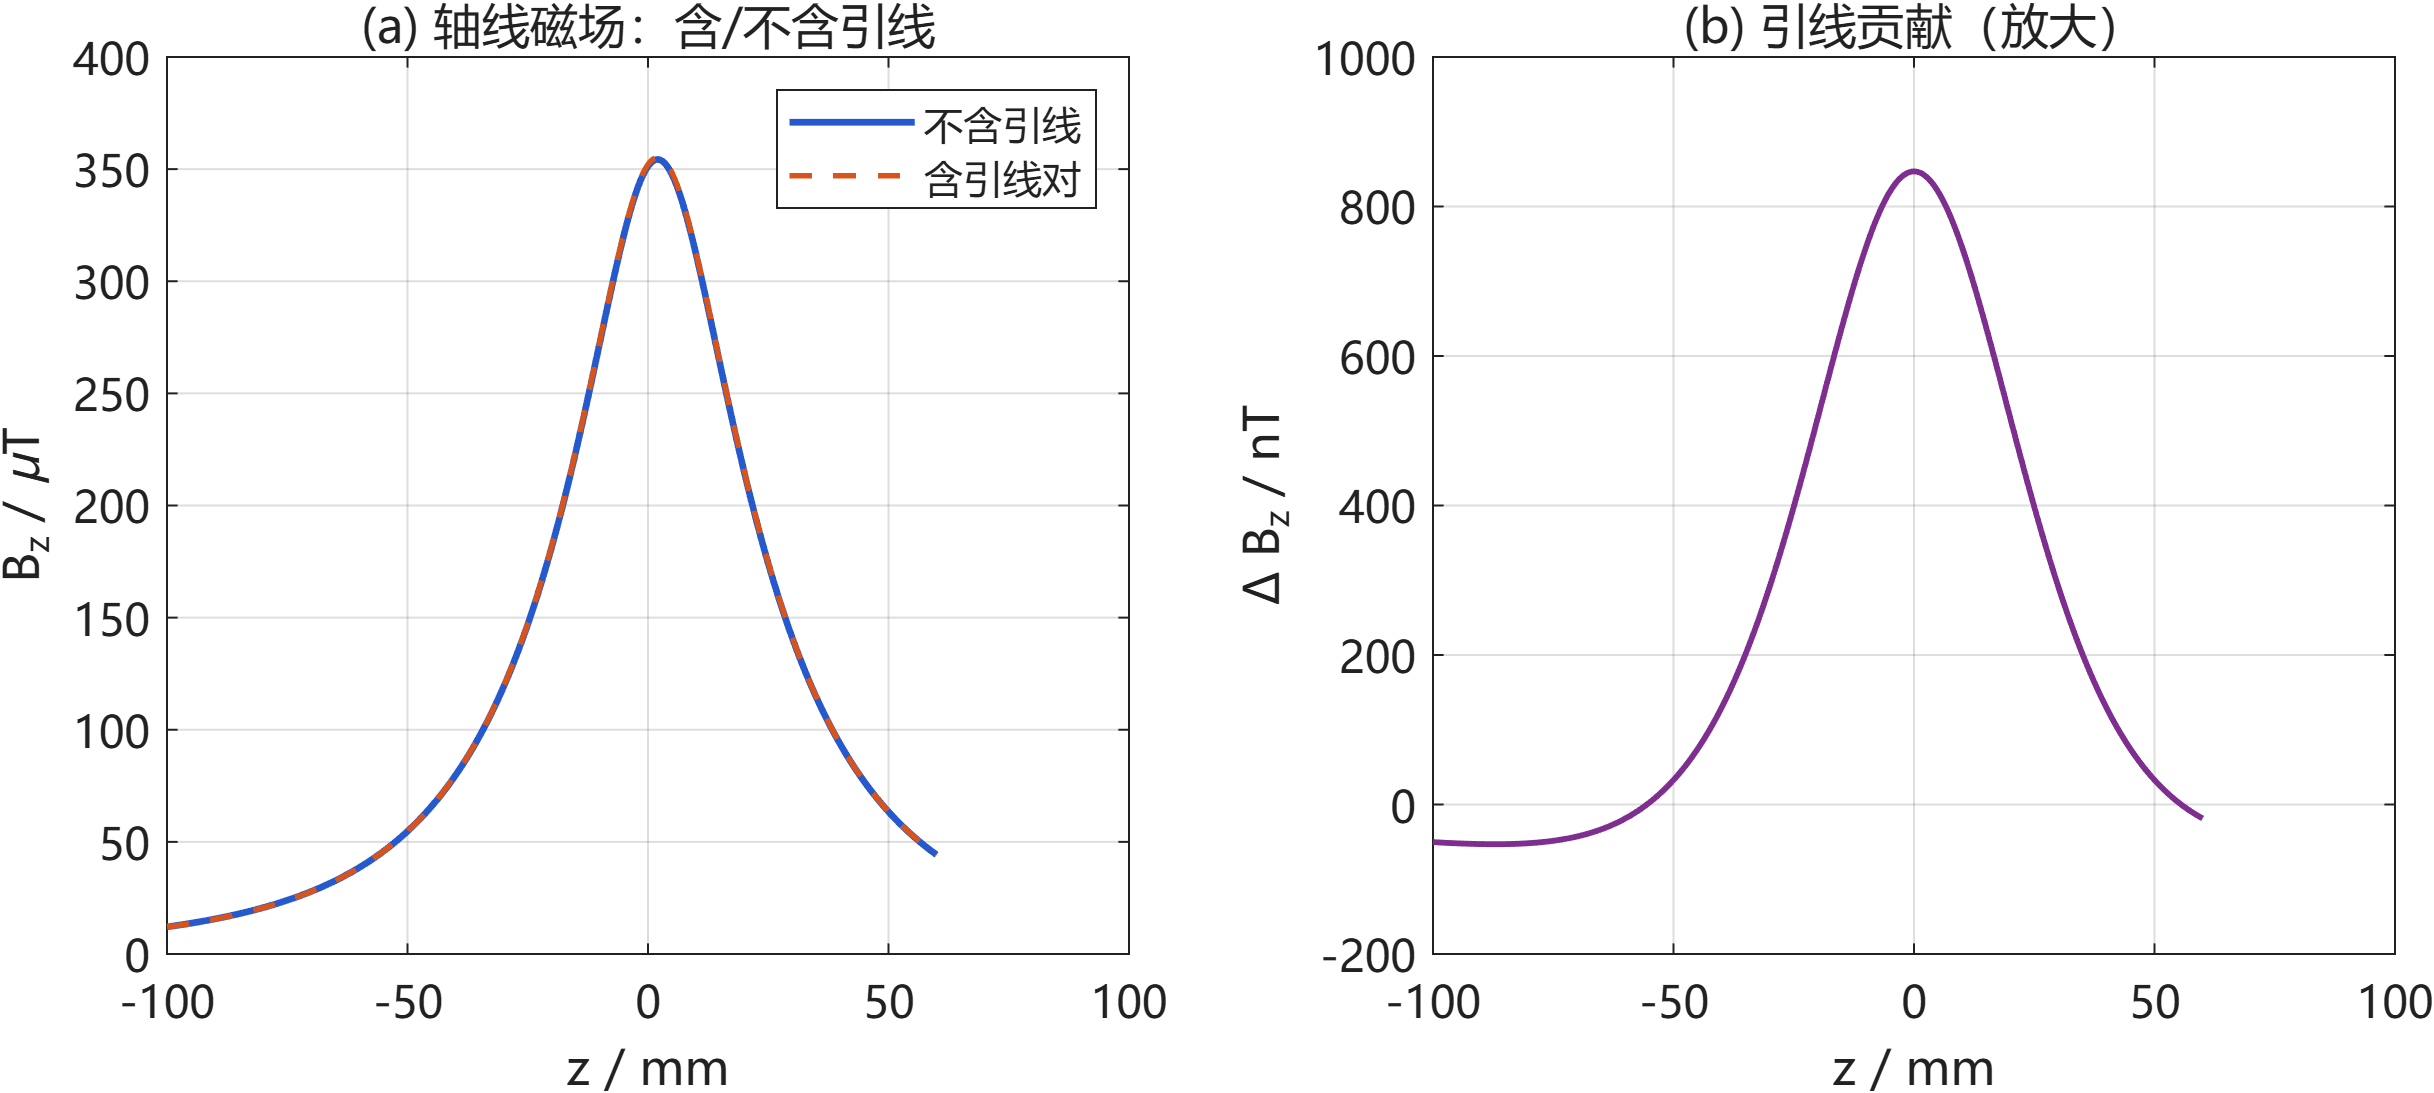
\includegraphics[width=0.98\textwidth]{fig06_leads_comparison.png}
  \caption{引线影响：含/不含引线的轴线磁场（a）及引线贡献（b）}
  \label{fig:leads}
\end{figure}

\subsection{电感与电阻估算}

按 Neumann 积分公式分段估算（互感项中点近似，单匝自感项用圆截面经验公
式），线圈电感 $L\approx\SI{19.5}{\micro H}$，直流电阻
$R\approx\SI{7.8}{m\Omega}$，导线总长 \SI{4.30}{m}。该电感量级与 TMS 设
备匹配回路（储能电容数毫法、触发晶闸管）的典型参数一致，说明图纸参数合
理；所有磁场结果按 $I$ 线性缩放，例如取脉冲峰值电流 \SI{5}{kA} 时线圈中
心磁感应强度约 \SI{1.76}{T}。

% ============================================================
\section{仿真软件仿真磁场及结果对比分析}\label{sec:fem}

\subsection{FEMM 有限元模型}

采用免费开源的轴对称静磁场有限元软件 FEMM 4.2\cite{meeker2019}建立对比
模型。圆形线圈及其磁场关于轴线旋转对称，故可用 $r$--$z$ 半平面的二维轴
对称模型代替三维模型，绕组以旋转体的矩形截面表示。模型设置如下：
（1）\textbf{求解域}：以线圈中心为圆心、半径 $r_0=\SI{1200}{mm}$（约 21
倍线圈半径）的半圆域，直边为对称轴；
（2）\textbf{绕组}：18 个 \SI{4}{mm}$\times$\SI{4}{mm} 矩形截面（对应
$\Phi 4$ 紫铜管，材料铜，$\mu_r=1$），截面中心与灯丝模型的匝中心重合，
各匝串联，电路电流 \SI{1}{A}；
（3）\textbf{外边界条件}：施加渐近混合边界条件
\begin{equation}
  \frac{1}{\mu_0}\frac{\partial A}{\partial n} + c_0 A = 0,
  \qquad c_0 = \frac{n}{\mu_0 r_0},
  \label{eq:asym}
\end{equation}
其中 $A$ 为矢量位，$n$ 为远场主导谐波衰减指数：轴对称偶极子场
$A\propto 1/r^2$，取 $n=2$。该条件近似「无穷远处 $A\to 0$」的开域解，避
免了简单截断（$A=0$ 或 $\partial A/\partial n=0$）造成的系统误差；
（4）\textbf{对称轴}：$r=0$ 上 $A=0$（轴对称问题 $A(0)=0$ 为精确条件，
且可消除轴上节点的数值噪声）；
（5）\textbf{网格}：一阶三角形单元，绕组及周围 \SI{130}{mm} 盒形区域内
空气网格尺寸 \SI{1}{mm}、外层空气 \SI{25}{mm}，共 91\,651 个单元、
46\,099 个节点。

建模中有三点经验值得说明：几何中边界 T 形相接处必须显式分段，否则网格剖
分与求解结果异常；轴线段需单独施加 $A=0$；通过脚本自动化建模时，FEMM
自带的 MATLAB 接口存在个别参数分支的书写缺陷，且混合边界条件须以含边界
类型参数的完整调用形式创建。

\subsection{对比结果}

图~\ref{fig:femm} 给出轴线磁场的对比：两条曲线在整个范围内重合，有限元
解相对数值解的均方根相对偏差为 0.44\%，最大 1.02\%；典型深度处的逐点偏
差列于表~\ref{tab:femm}，均在 $\pm 0.4\%$ 以内。$z=\SI{-10}{mm}$ 平面径
向分布的对比：$B_z$ 峰值偏差 +0.29\%；在 $|B_z|$ 大于 5\% 峰值的区域内
逐点偏差均方根 1.96\%（最大偏差位于绕组外侧 $B_z$ 过零点附近，该处场值
本身趋近于零，相对偏差自然放大；以峰值归一的全量程最大偏差仅 0.93\%）。

\begin{table}[htbp]
  \centering
  \caption{轴线磁场：MATLAB 数值解与 FEMM 有限元解的对比（\SI{1}{A}）}
  \label{tab:femm}
  \begin{tabular}{cccc}
    \toprule
    深度 $z$ / mm & 数值解 / \si{\micro T} & FEMM / \si{\micro T} & 相对偏差 \\
    \midrule
    0（线圈中心） & 351.29 & 350.55 & $-0.21\%$ \\
    $-10$ & 272.87 & 273.38 & $+0.19\%$ \\
    $-20$ & 181.67 & 181.39 & $-0.16\%$ \\
    $-30$ & 119.26 & 119.58 & $+0.27\%$ \\
    $-40$ & 79.77  & 80.07  & $+0.37\%$ \\
    $-50$ & 54.75  & 54.58  & $-0.30\%$ \\
    \midrule
    均方根相对偏差 & \multicolumn{3}{c}{0.44\%（最大 1.02\%）} \\
    \bottomrule
  \end{tabular}
\end{table}

\begin{figure}[htbp]
  \centering
  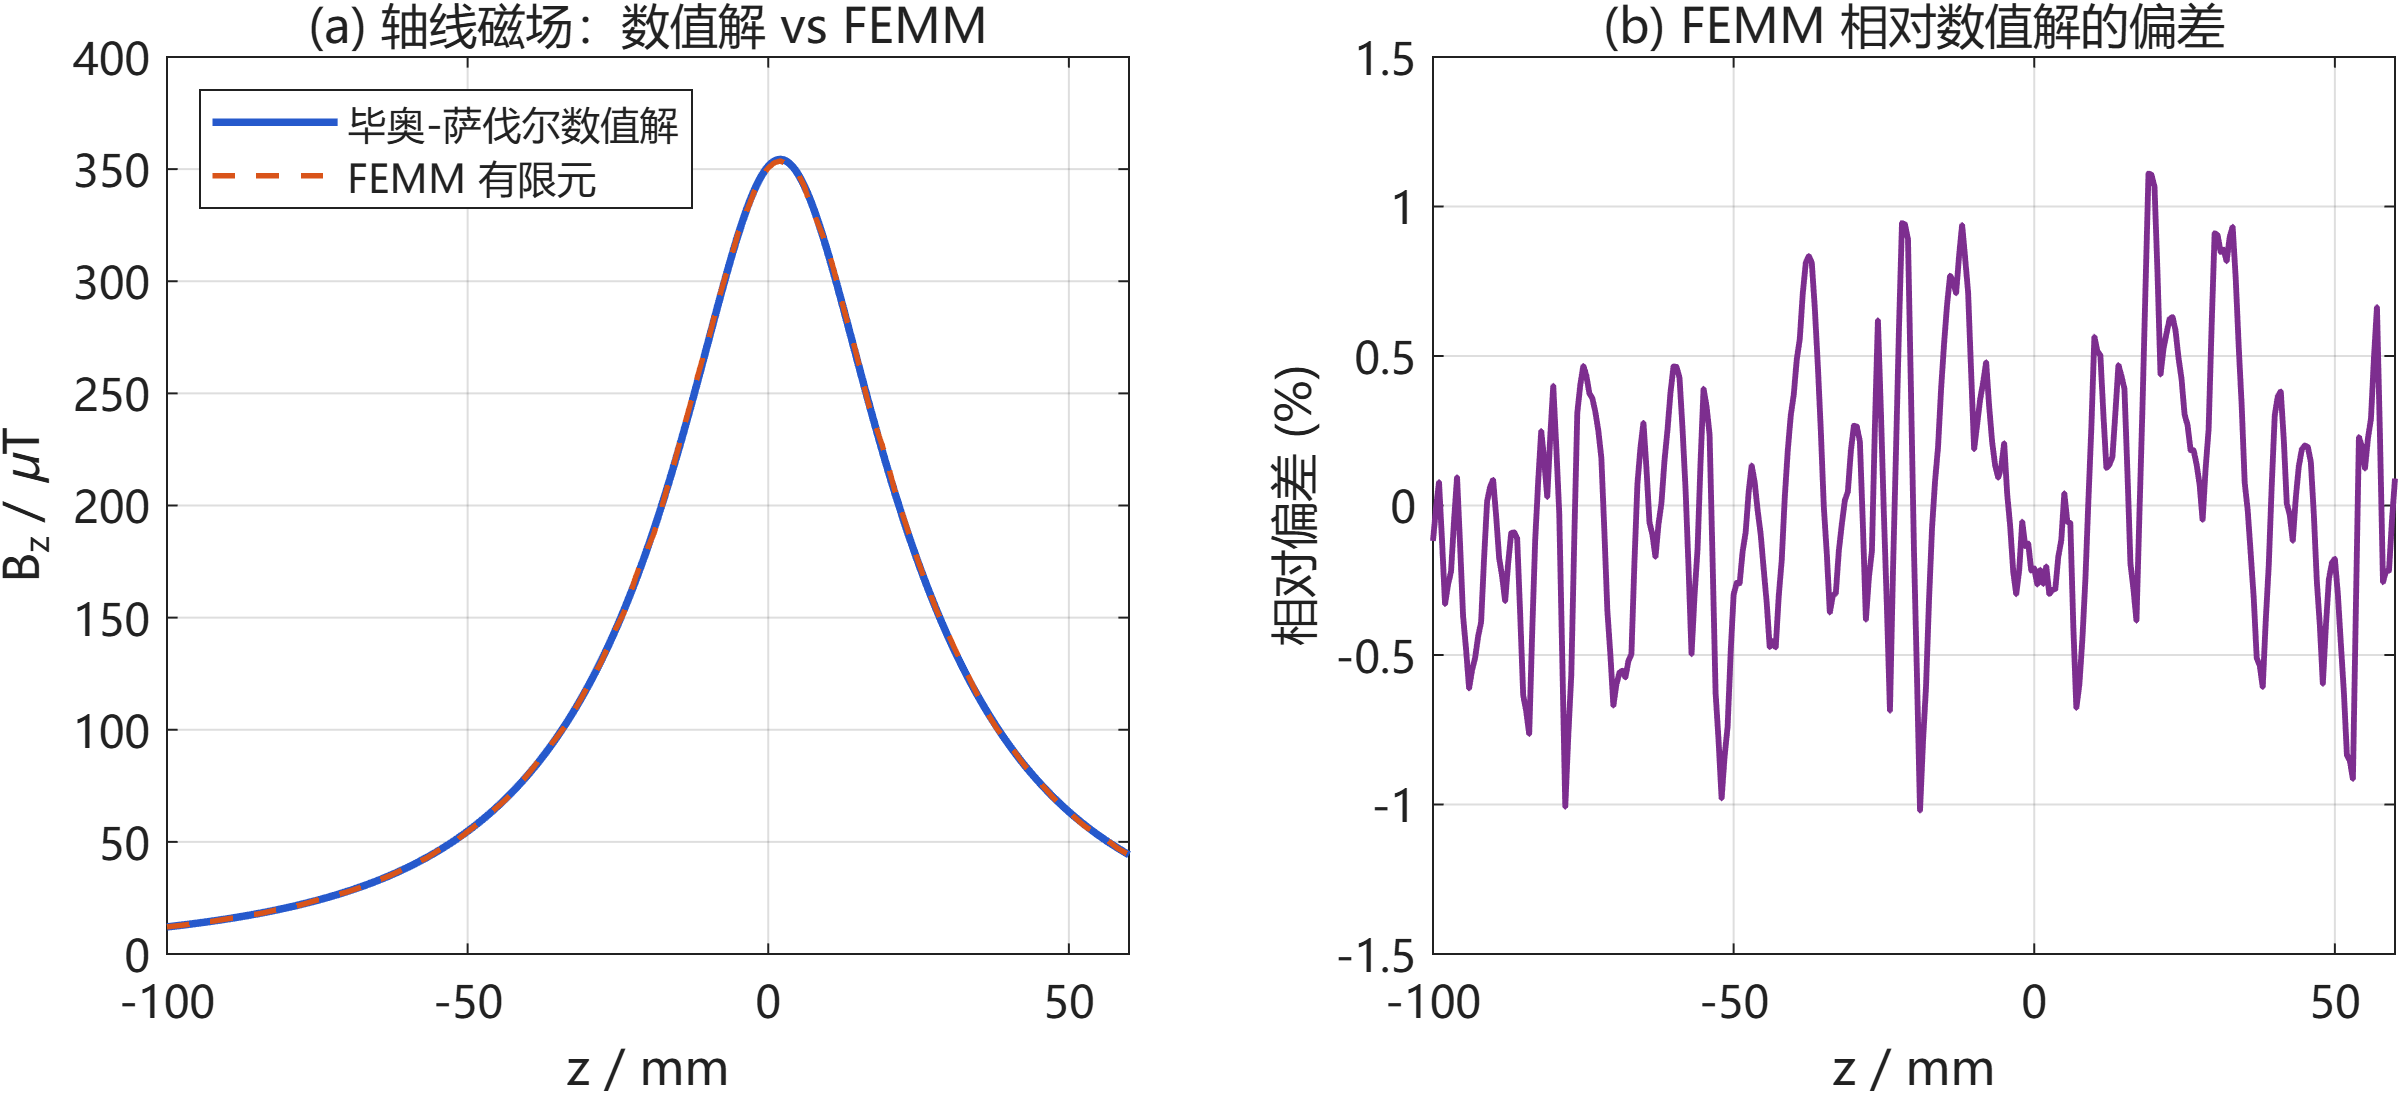
\includegraphics[width=0.98\textwidth]{fig08_femm_comparison.png}
  \caption{轴线磁场：MATLAB 数值解与 FEMM 有限元解的对比（a）及相对偏差（b）}
  \label{fig:femm}
\end{figure}

\subsection{偏差来源分析}

两种方法在全部对比点上的偏差不超过 $\pm 1\%$，来源包括：
（1）\textbf{电流分布模型差别}：数值解将电流集中为灯丝，有限元模型为
\SI{4}{mm}$\times$\SI{4}{mm} 均匀分布截面。对分块截面模型做解析积分表明
该差别对轴线磁场的影响小于 0.15\%，是最主要的系统偏差来源；
（2）\textbf{有限元离散误差}：一阶三角形单元内磁位线性、磁感应强度为分
片常数，绕组附近场梯度大处误差增大（对应径向分布过零点附近的局部偏
差）；
（3）\textbf{开域边界近似}：渐近边界条件只匹配远场主导谐波，其残差随距
离衰减，在 \SI{1200}{mm} 外边界下对关心区域的影响已可忽略；
（4）\textbf{几何离散}：数值解以 240 段/匝的弦线代替螺旋弧线（贡献约
$2\times10^{-4}$）。

两种方法原理完全独立——其一基于宏观电磁场的积分定理（毕奥--萨伐尔定律）
逐单元精确叠加，其二基于微分方程（磁位泊松方程）的变分离散——在小于
1\% 的水平上相互吻合，验证了计算模型与程序实现的正确性。

% ============================================================
\section{结论}\label{sec:conclusion}

本文针对课题一的圆形 TMS 线圈（平面螺旋、双层 9 匝、外径
\SI{115}{mm}、内径 \SI{30}{mm}），完成了理论建模、MATLAB 数值计算与有限
元仿真对比，主要结论如下：

（1）基于毕奥--萨伐尔定律与直线单元闭式磁场公式建立了线圈磁场计算模型，
辅以 AGM 完全椭圆积分自实现，无工具箱依赖。模型经双重解析验证：轴线磁场
与多匝圆环解析解最大偏差 0.27\%，单匝离轴场与椭圆积分精确解峰值归一偏差
$2.3\times10^{-4}$。

（2）归一化电流 \SI{1}{A} 下，线圈中心磁感应强度 \SI{351.29}{\micro T}
（峰值 \SI{354.34}{\micro T} 位于双层绕组之间）；线圈下方 \SI{10}{mm} 处
峰值衰减至 77.7\%，半衰深度约 \SI{27}{mm}；径向半高全宽由绕组内的
\SI{30}{mm} 增至深处的约 \SI{70}{mm}。圆形线圈磁场衰减快、聚焦性随深度
变差，验证了其作为 TMS 基础构型的局限性与改进方向。引线（反流对）对磁
场的贡献不超过 0.42\%，可忽略。估算电感 \SI{19.5}{\micro H}、直流电阻
\SI{7.8}{m\Omega}，与 TMS 设备参数匹配。

（3）FEMM 轴对称有限元模型（91\,651 个一阶三角形单元，渐近混合边界条
件）与数值解对比：轴线磁场均方根相对偏差 0.44\%、最大 1.02\%，径向分布
峰值偏差 0.29\%。两种独立方法在 1\% 精度内相互验证，偏差主要来自灯丝近
似与一阶单元离散，均远小于工程精度需求。

% ============================================================
\bibliographystyle{unsrt}
\bibliography{ref}

\end{document}
